% \iffalse
\let\negmedspace\undefined
\let\negthickspace\undefined
\documentclass[journal,12pt,twocolumn]{IEEEtran}
\usepackage{amsmath}
\usepackage{graphicx}
\newtheorem{theorem}{Theorem}[section]
\newtheorem{problem}{Problem}
\newtheorem{proposition}{Proposition}[section]
\newtheorem{lemma}{Lemma}[section]
\newtheorem{corollary}[theorem]{Corollary}
\newtheorem{example}{Example}[section]
\newtheorem{definition}[problem]{Definition}
\newcommand{\BEQA}{\begin{eqnarray}}
\newcommand{\EEQA}{\end{eqnarray}}
\newcommand{\define}{\stackrel{\triangle}{=}}
\newtheorem{rem}{Remark}
\begin{document}
\parindent 0px
\bibliographystyle{IEEEtran}
\title{Assignment 10.5.3\_18Q}
\author{EE23BTECH11028 - Kamale Goutham$^{}$% <-this % stops a space
}
\maketitle
\newpage
\bigskip
\section*{Question}
A spiral is made up of successive semicircles,with centres alternately at A and B,starting with centre at A,of radii $0.5cm,1.0cm,1.5cm,2.0cm$,... as shown in Fig.$5.4$.what is the total length of such a spiral made up of thirteen consecutive semicircles?(Take $\pi=\frac{22}{7}$)\\
\begin{figure}[h]
  \centering
  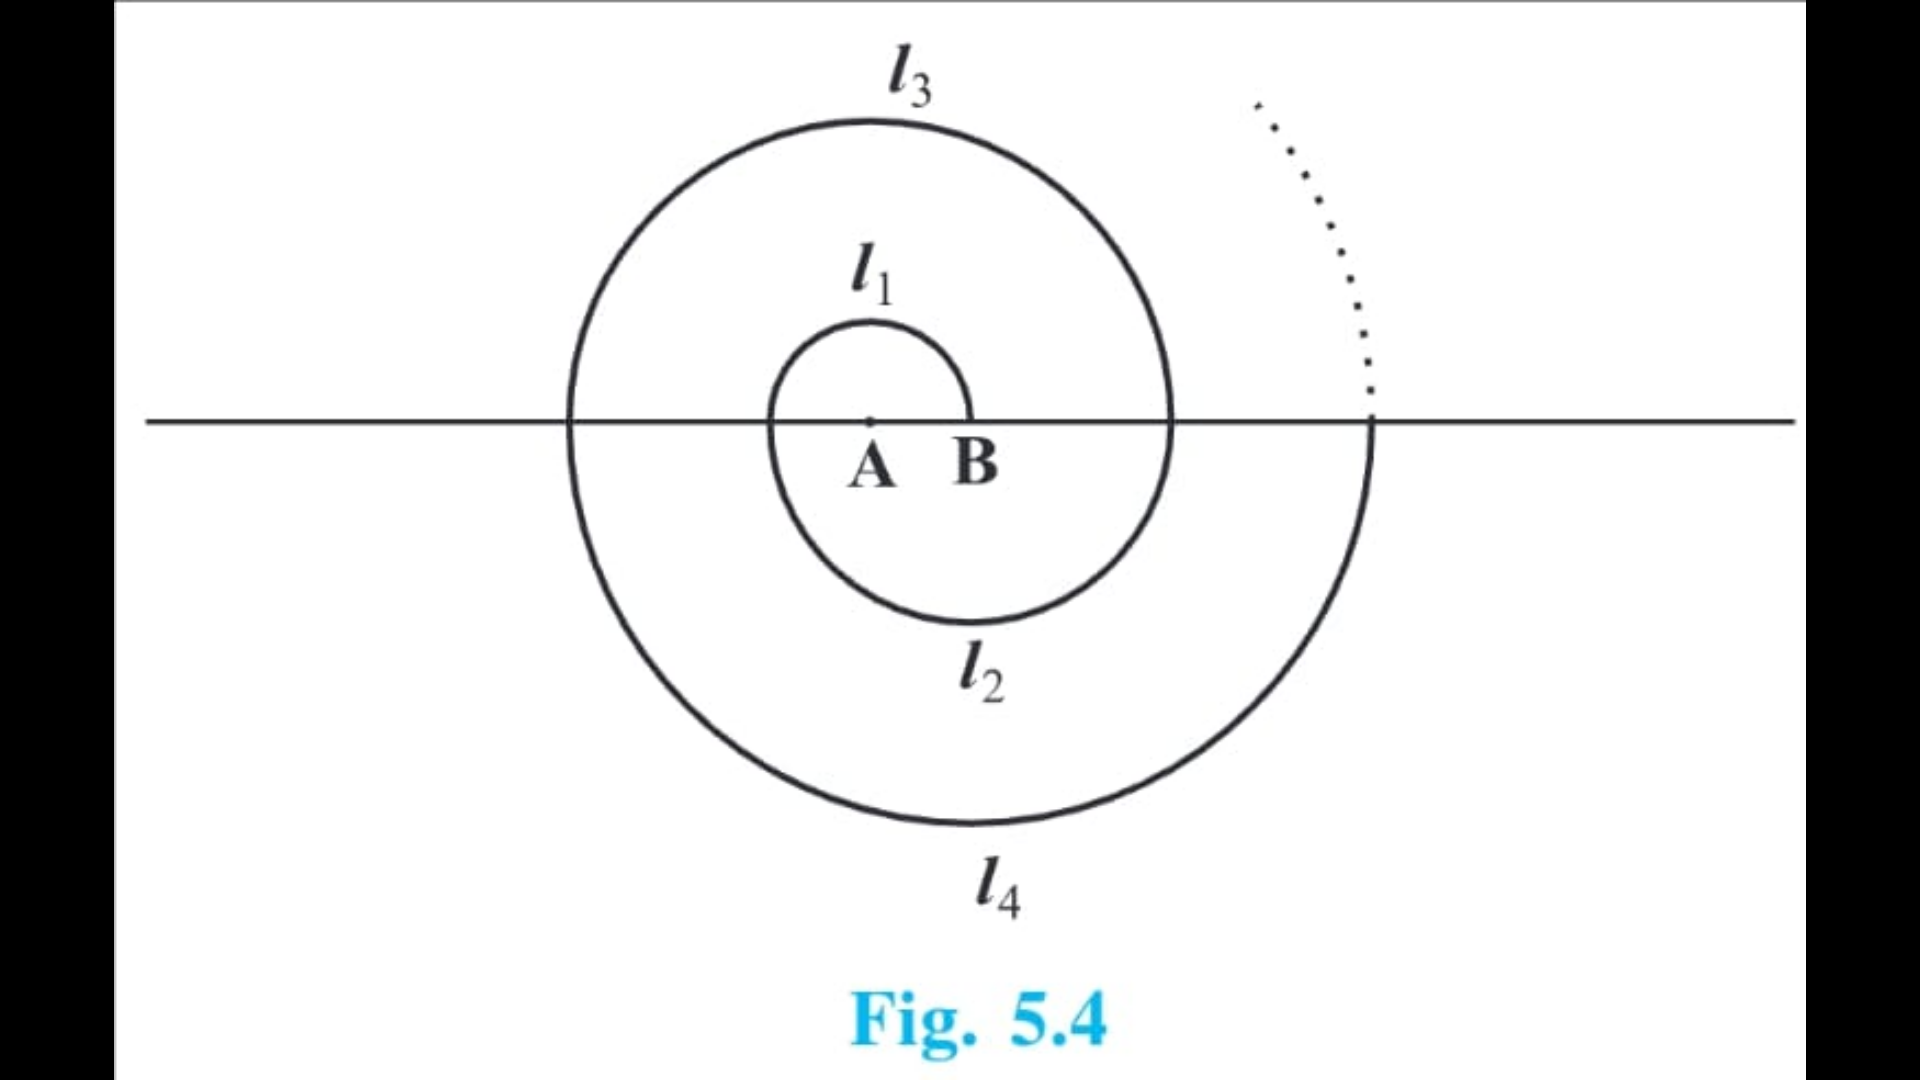
\includegraphics[width=\columnwidth]{Fig. 5.4.png}
  \caption{$5.4.$}
\end{figure}
\end{document}
